\chapter{Non-RDB Example: Redis}

Redis, short for \textit{REmote DIctionary Server}, is an open-source in-memory distributed key-value database.

The community version of Redis is free of cost and can be installed on multiple platforms. Redis Cloud, on the other hand, is a paid service with additional features and can be deployed on various cloud platforms such as AWS, Azure, and Google Cloud.

\section{Brief Introduction to Redis}

Redis is an open-source in-memory distributed database. It is a NoSQL database and does not structure and store data in tables. Unlike MongoDB, which stores data using self-contained documents, Redis stores data in key-value pairs. Redis is renowned for its support of in-memory data storage, significantly speeding up data storage, query, and processing. As a result, it is often used as a lightweight data caching tool or a message broker.

The features of Redis are summarized as follows:
\begin{itemize}
	\item In-memory storage: This speeds up reading and writing operations.
	\item Persistence: While primarily an in-memory database, Redis offers various ways to persist data on disk without significantly compromising performance.
	\item Complex data structures and associated atomic operations: Though Redis is a key-value store, it supports more complex data structures than just simple key-value pairs.
	\item High availability via replicas: Redis can create replicas to ensure high availability.
	\item Distributed storage via horizontal partitioning: Redis supports horizontal partitioning for distributed storage.
	\item Lightweight: Redis is designed to be lightweight, making it efficient and easy to use.
\end{itemize}

A potential drawback of Redis is that when it is used in-memory, the data may be lost in the event of a system shutdown. For this reason, a popular way of using Redis is to let it sit between the user and a persistent database running in the backend. In this architecture, Redis serves as a fast-responding replica to enhance the user experience. When the data to retrieve is in Redis, the system does not need to query the backend database and it can return the result in milliseconds, which otherwise would have cost hundreds or thousands of milliseconds.

\section{Installation}

To install Redis on a Linux machine, simply use the package manager of the machine. For example, for RHEL, do the following
\begin{lstlisting}
$ sudo dnf install redis
\end{lstlisting}
to install Redis, and use
\begin{lstlisting}
$ redis-server
\end{lstlisting}
to start the Redis server. Upon starting of Redis, the port number and the process id will pop up. By default, it runs on port $6379$.

To login to Redis on the host machine, simply use
\begin{lstlisting}
$ redis-cli
\end{lstlisting}
to open the CLI to the database. The CLI prompt that looks like
\begin{lstlisting}
127.0.0.1:6379>
\end{lstlisting}
shall show up, from where the user can type in the commands. In the rest of this chapter, we will use \verb|>| as the prompt indicator in the CLI.

\section{Basic Operations}

Basic operations such creating, querying and removing key-value pairs, arrays, sets, and hashes are introduced as follows.

\subsection{Key-Value Pair Operations}

Redis utilizes a key-value based data structure in the database. Therefore, the basic operations of Redis include creating, querying and deleting key-pair values. Notice that Redis CLI commands are not case sensitive in general, though in the examples below upper-case commands are used.

To set or overwrite a key-pair value, use
\begin{lstlisting}
> SET <key> <value>
\end{lstlisting}
where notice that both the key and the value are to be interpreted as strings. If a value is composed of multiple words in its string, use quotation marks to wrap the content.

To retrieve the value of a key, use
\begin{lstlisting}
> GET <key>
<value>
\end{lstlisting}
Notice that the value is usually returned as a string datatype, even if it is a number. If the key does not exist, it would return \verb|(nil)|.

To check whether a key exists or not, use
\begin{lstlisting}
> EXISTS <key>
\end{lstlisting}
and it will return either \verb|(integer) 1| or \verb|(integer) 0| to indicate whether the key exists or not respectively.

Finally, to remove a key, use
\begin{lstlisting}
> DEL <key>
\end{lstlisting}

To retrieve all the keys in the database, use
\begin{lstlisting}
> KEYS *
\end{lstlisting}

To remove all the keys, use
\begin{lstlisting}
> FLUSHALL
\end{lstlisting}

It is possible to set TTL for a key, so that after a certain amount of time, the key-value pair would be removed automatically. To set TTL for a key, use
\begin{lstlisting}
> EXPIRE <key> <seconds>
\end{lstlisting}
where \verb|<key>| is an existing key. To check the TTL of a key, use
\begin{lstlisting}
> TTL <key>
\end{lstlisting}
where notice that a TTL of \verb|-1| means that the key lives indefinitely, and \verb|-2| the key does not exist probably because its TTL has expired. 

To set TTL of a key upon it is created, use
\begin{lstlisting}
> setex <key> <seconds> <value>
\end{lstlisting}

\subsection{Array Operations}

Redis allows storing array as the value of a key, and it supports array-based operations.

To create or append an array, use
\begin{lstlisting}
> lpush <key> <value last> ... <value first>
\end{lstlisting}
Note that when using \verb|lpush|, the last item in the above input will be treated as the first element. This is because it pushes a new item to the left (beginning) of an array. To push new items from the right (end) of an array, use \verb|rpush| instead as follows.
\begin{lstlisting}
> rpush <key> <value first> ... <value last>
\end{lstlisting}

To retrieve items from an array, use
\begin{lstlisting}
> lrange <key> <start index> <stop index>
\end{lstlisting}
which returns elements indexed from the start index to the stop index, both ends included. Notice that the first element in the array is indexed $0$. When the stop index is set to $-1$, all items from the start index to the end of the array is to be returned. Hence, to return everything in an array, set the start and stop indexes to be $0$ and $-1$ respectively.

Finally, to remove an item from an array from its two ends, use
\begin{lstlisting}
> LPOP <key>
<first value>
\end{lstlisting}
or
\begin{lstlisting}
> RPOP
<last value>
\end{lstlisting}
which returns and at the same time removes the first or the last item in the array respectively.

\subsection{Set Operations}

It is not convenient to trace whether an item exists or not in an array introduced above. For that use case, consider using sets instead. A set is a collection of elements where each value is unique and has no orders.

To create and add items to a set, use
\begin{lstlisting}
> SADD <key> <value> <value> ...
\end{lstlisting}
where \verb|<key>| is the name of the set. Notice that elements in a set cannot duplicate, otherwise it will trigger an exception.

To check whether an item is in a set, use
\begin{lstlisting}
> SISMEMBER <key> <value>
\end{lstlisting}
which returns either $0$ (not exist) or $1$ (exist).

To remove an item from a set, use
\begin{lstlisting}
> SREM <key> <value> <value>
\end{lstlisting}

To retrieve all the elements from a set, use
\begin{lstlisting}
> SMEMBERS <key>
\end{lstlisting}

\subsection{Hashes}

Hashes allows the user to store objects, i.e., a set of key-value pairs. Note that nested object is not supported.

To create, overwrite or add fields to a hash, use
\begin{lstlisting}
> HSET <key> <field> <value> <field> <value> ...
\end{lstlisting} 

To retrieve a hash or a particular field of a fash, use the following.
\begin{lstlisting}
> HGET <key> <field>
\end{lstlisting}
returns the value of the selected field of a hash, and
\begin{lstlisting}
> HGETALL <key>
\end{lstlisting}
returns all field-value pairs of a hash.

To check whether a field has been defined for a hash, use
\begin{lstlisting}
> HEXISTS <key> <field>
\end{lstlisting}
which returns either $0$ (not exist) or $1$ (exist).

To delete fields from a hash, use
\begin{lstlisting}
> HDEL <key> <field> <field> ...
\end{lstlisting}
Note that if all the fields of a hash are deleted, the hash itself will disappear.

\section{Redis in Practice}

A commonly seen architecture of implementing Redis is given in Fig. \ref{ch:database:redisarchitecture}. The idea is that the program that needs to retrieve the information from the backend persistent database should search for the in-memory Redis database first. If the data is already stored in Redis and has not expired its TTL, the program will not query data from the backend database, but to directly retrieve data from Redis. Redis plays as a replica of the database to speed up reading.

\begin{figure}[htbp]
	\centering
	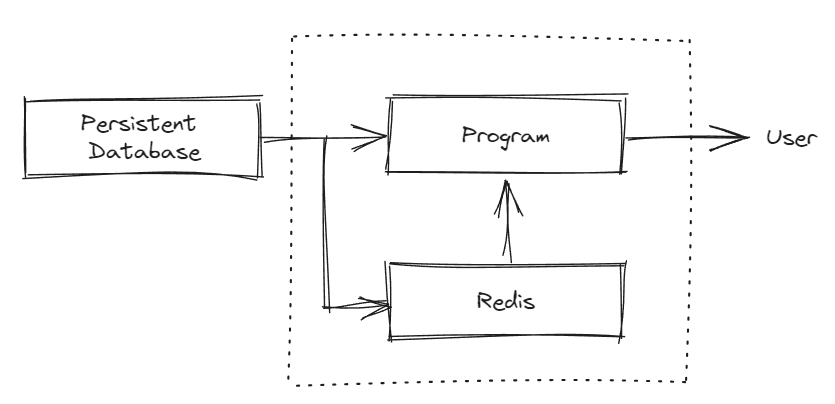
\includegraphics[width=0.8\textwidth]{chapters/part-3/figures/redis_architecture.png}
	\caption{A commonly seen architecture of implementing Redis.} \label{ch:database:redisarchitecture}
\end{figure}

Other than replica of database for reading, the following gives a list use cases where Redis may be helpful:
\begin{itemize}
	\item Data caching
	\item Message brokering
	\item Distributed locking
	\item Real-time data streaming, processing and analyzing
\end{itemize}

In addition to Redis CLI which a user can use to interact with Redis from the console, Redis also supports the following main languages. The program in these languages can connect to Redis via the Redis client.
\begin{itemize}
\item Python
\item C\# / .NET
\item Node.js
\item Java
\item Go
\end{itemize}
More information is given at \cite{redis2024client}.
